\section{Results}\label{sec:results}

With a complete experimental set-up, benchmark performance was established using the simple models ranging from the
SVM to the basic fully-connected network, at around 70-80\%.
Both 2 dimensional and 3 dimensional convolutional networks were able to surpass the benchmarks,
attaining 95\%+ and 90\%+ accuracy respectively.

The stretch goal of region highlighting using unsupervised segmentation proved infeasible for this project timeframe, given
the challenges overcome with the 3d convolutional model architecture.

\subsection{Model Architecture}\label{subsec:model-arch}

the project explored minimally the hyperparameters of the chosen model architectures
chiefly was finding the right learning rate for the given normalized data to the model
typically 1e-2 to 1e-4 worked, with 1e-3 being best, and decay being very very helpful
model quite sensitive to adjustments

- scheduler / hyperparams / diff architectures (just go with res3d, res2d+1d, mix three types

\subsection{Scope of Number of Subjects}\label{subsec:num-subjects}

inclusion of more ppts/subjects means more training time (val/test are of same patients,
hence more individual brain shapes means more general, but longer to learn)
20 epochs to see liftoff of 55% with 10 ppts, vs quicker with 6ppts

 \begin{figure}
  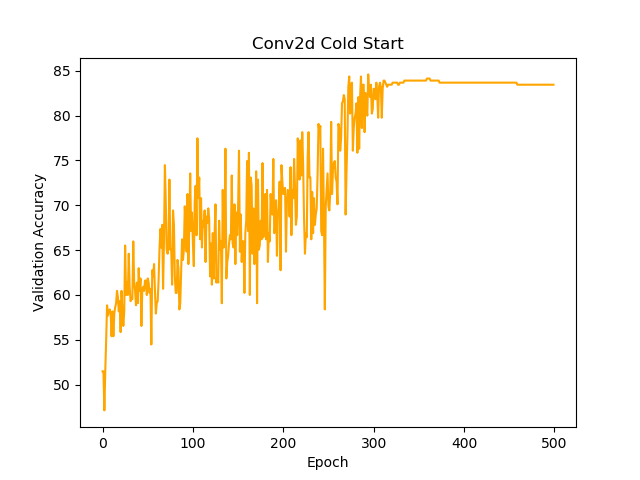
\includegraphics[width=\linewidth]{images/2d_cold.png}
  \caption{Cold-Start 2D Training Progress}
  \label{fig:2d_cold}
\end{figure}

\subsection{Warm Starts}\label{subsec:warm-starts}
saving model parameter dict, loading and training again
wowee good stuff, hope to use a LR scheduler in the future to try to control this better?
surprisingly bad results on warm starting expansion to new subjects - old same subjects takes a little while to stabilize
but it gets back to 83% without much fuss, probably LR is a little high to start with and the decay helps a lot.
bounces down for a while, bounces up for a while. breaking 90% which is very cool, might mean warm start has best potential

 \begin{figure}
  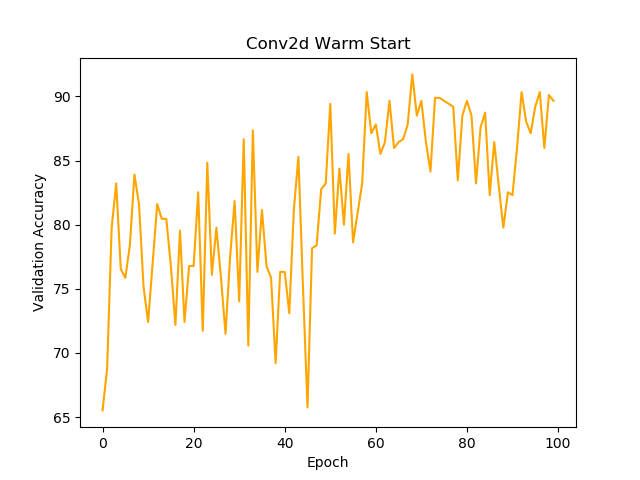
\includegraphics[width=\linewidth]{images/2d_warm.png}
  \caption{Warm-Start 2D Training Progress}
  \label{fig:2d_warm}
\end{figure}

\subsection{3 Dimensions}\label{subsec:3-dimensions}
- 3d CNN - typically meant for video classification using time as the third axis,
here we are not using time, though that is a dimension we have access to,
though doesn't make sense for this experiment/project to try to add in
- https://pytorch.org/docs/stable/torchvision/models.html#video-classification


okay it works, and has potential, certainly given the data is richer to be the best, but wow it's frustratingly slow
findings: 3d is cool, but crazy prohibitively slow and not much better than 2d without more refinements. IMHO theres
promise still in exploring it, but given the inexcusable runtime and datasize 2d is probably worth more investment
unless better hardware or serious effort is expended in getting it differentiable

 \begin{figure}
  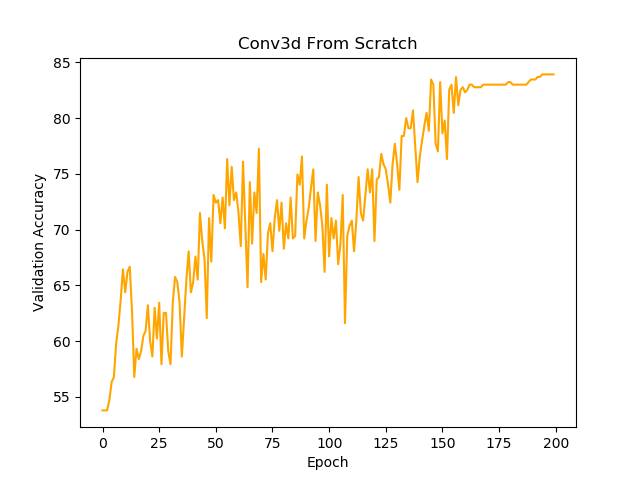
\includegraphics[width=\linewidth]{images/3d_cold.png}
  \caption{Cold-Start 3D Training Progress}
  \label{fig:3d_cold}
\end{figure}
wrestling with memory constraints (batch size / 3d data huge for cpu/gpu, dataset pretty large in general for ram) slow learning, tapering off learning
different styles of 1d (unfurl 3d, 2d) 2d (mean flattened, one slice) 3d (scale, orig)
LR explorations

future works
better gpu / computer might be important, the 3d models are real fucking beasts to train, and their data is large as fuck
model ensemble (free extra few percent perf)



"none of my alterations to the model architecture worked that well, most did nothing, a few broke things, could still poke around more though"
graphs from 2d training, 3d takes legit 2-3 hours for 200 epochs on 6 subjects with 5./6 & 7. / 2.
batch_size and interpolation hard to juggle too?
3d feels like "luck" plays a big part of getting training to catch/start
seems like scaling down is pretty important and I have better luck with larger batch sizes (meaning scale down is crucial) wonder if aggressive scale down is worthwhile, like over 3./4, image gets real grainy real fast)

cut batch size to avoid scaling down images (TRIED NO BUENO?)

\subsection{Performance Measures}\label{subsec:performance}

 % P-R-F1-S
\begin{center}
 \begin{tabular}{||c c c||}
 \hline
 - & Nonfood & Food \\ [0.5ex]
 \hline\hline
Precision & 0.949074 & 0.958904 \\
 \hline
Recall & 0.957944 & 0.950226 \\
 \hline
F1 & 0.953488 & 0.954545 \\
 \hline
Support & 214 & 221 \\ [1ex]
 \hline
\end{tabular}

 % ROC-AUC / ACC
\end{center}
\begin{center}
 \begin{tabular}{||c c||}
 \hline
 ROC-AUC & Accuracy \\ [0.5ex]
 \hline\hline
  0.9847 & 0.954 \\ [1ex]
 \hline
\end{tabular}
\end{center}

Can get a little higher but these are already encouraging numbers (96 seen) often the model starts leaning a little
one way or the other and this was one of the most balanced runs I've seen

I'm a little unclear about the reliability of my data labeling, so I'm happy with this result, I'd be stoked
to reproduce on 3d, and trusting the model this much, open the door to segmentation
